%==== Document Setup (usthesis)======================================
\documentclass[report,                       %... Document type
               12pt,oneside,openany,a4paper, %... Layout
               a5block,                      %... A5 type block
               english,english,         %... Afrikaans default language
               ]{usthesis}

%
% PLEASE read the USthesis documentation for the class options
% and how to set line and paragraph spacing
%

%==== Language setup ================================================
 \usepackage[latin1]{inputenc}%................... Recognizes �, �, etc
 \usepackage{babel}%.............................. Language setup

%==== Math setup ====================================================
 \usepackage{amsmath}%............................ Advanced math (before fonts)
 %\usepackage{amssymb}%............................ AMS Symbol fonts

%==== Font setup (default is Computer Modern) =======================
 \usepackage[T1]{fontenc}%........................ Type 1 fonts
 \usepackage{textcomp}%........................... Additional text character
 \usepackage{bm}%................................. Bold math symbols (after fonts)

%==== Ref's, Bib's and Nomencl ======================================
 \usepackage{usnomencl}%.......................... List of symbols (in usthesis pack)
 \usepackage{usbib}%.............................. Bibliography    (in usthesis pack)
    \bibliographystyle{usmeg-a}
    \renewcommand\bibfont{\small}

    %% For usmeg-a, the bib is a list of references. If you
    %% are using usmeg-n comment out the following lines
    \addto{\captionsafrikaans}{\renewcommand{\bibname}{Lys van Verwysings}}
    \addto{\captionsenglish}{\renewcommand{\bibname}{List of References}}

%==== Graphics and Color ============================================
\usepackage{graphicx}%........................... Graphicx loaded in usthesis
\usepackage{color}%.............................. Color setup
\usepackage{float}%.............................. To tell an image exactly where you want it placed
%==== Additional USthesis packages ==================================

\usepackage{ussummary}%.......................... Mech Eng summary page (in usthesis pack)

%==== Background image ====================================================
\usepackage{eso-pic}
\newcommand\BackgroundPic{%
\put(0,0){%
\parbox[b][\paperheight]{\paperwidth}{%
\vfill
\centering

\includegraphics[width=\paperwidth,height=\paperheight,keepaspectratio]{background.png}%
\vfill
}}}
%==== Local Defs ====================================================
\makeatletter

%
% Please insert user defined commands here
% and NOT in the document itself!
%

\makeatother
%==== Title Page ====================================================

\title{Stochastic inversion of fire test data \\
for the T-dependant thermal diffusivity of SA pine}

\author{L.\ Stewart}
       {Liza Stewart\\
           21555575}

\subject{Project(Civil Engineering)458}
        {Project(Civil Engineering)458}

\ReportDescript{Project Proposal}

\address{Department Civil Engineering,\\
         University of Stellenbosch,\\
         Privatebag X1, Matieland 7602.}

\studyleader{Prof N\ de Koker}

\setdate{08}{2021}

%====================================================================%
%                 T H E   M A I N   D O C U M E N T                  %
%====================================================================%
\begin{document}
%\AddToShipoutPicture*{\BackgroundPic}
\frontmatter%========================================================

\TitlePage
\CopyrightPage
%\include{verklaring}
%\include{opsomming}
%\include{uittreksel}
\tableofcontents
\listoffigures
\listoftables
\include{nomenkl}

\mainmatter%=========================================================

\numberwithin{equation}{section}%(from amsmath)
\numberwithin{figure}{section}  %
\numberwithin{table}{section}   %

 \chapter{Introduction}
\section{Background and Motivation}

Traditionally the thermal diffusivity, otherwise referred to as the $\alpha$-value, of timber is based simply off the EN 1995:1-1-2004 or similar standards.
This research project will aim to obtain the thermal diffusivity of cross laminated SA-Pine timber by further analysing data obtained by S van der Westhuisen for his study of the samples' charring rate.

The thermal diffusivity of timber is a unobservable quantity that cannot be measured by itself, instead it is related to measurements of temperature and time through differential models. 
When heat diffusion is calculated using Finite Element methods the process is usually simplified to a linear problem(Fish). 
Due to the changes in thermal diffusivity of timber with temperature, as can be seen in EN 1995:1-1-2004(pg number), the diffusivity cannot be linearly modelled. 
Therefore problem lends itself to being analysed by inversion techniques. 
The aforementioned approach will allow us to obtain information about the diffusivity based on the combination of the information assumed prior to measuring, further referred to as the prior, and the measured data. 
Using statistical inversion leads to a probability distribution that provides us with a collection of diffusivity estimates and their corresponding probabilities.\citet{Lin:1997}


%This will be done by adjusting a finite element model created by Dr. N de Koker into a function. This function will be used in a Bayes model to solve for the temperature dependant thermal diffusivity.
\section{Aim and objectives}
During the course of the project the student will aim to meet the following objectives:
\begin{enumerate}
 \item Modify a Finite Element Model into an accurate and effective function.
 \item Compare the model data to the actual acquired data.
 \item Solve for the thermal diffusivity using Bayes' theorem of inverse problems
 \item Evaluate and explore the posterior probability distribution using the following methods:
 	\begin{enumerate}
 		\item Maximum a Posteriori
 		\item Markov-Chain Monte Carlo 	
 	\end{enumerate}
\end{enumerate}

\section{Literature Review}
	\subsection{K- value}
%	
%	\begin{figure}
%	\label{kvalue_fig}
%	\begin{center}
%	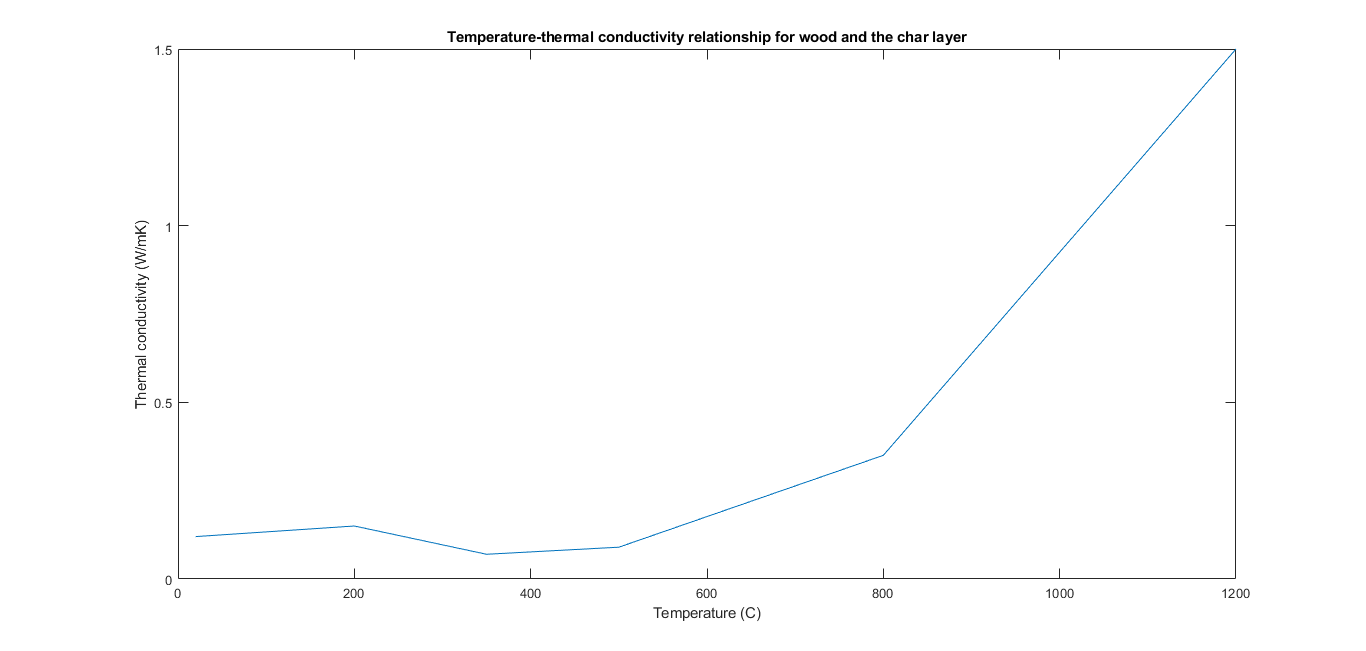
\includegraphics[width = 3]{kvalues_euro.png}
%	\end{center}
%	\end{figure}
	
	\subsection{Bayes' theorem of inverse problems}
%	Statistical and Computational Inverse problems by Kaipio and Somersalo Chapter 3
% 	The Bayesian approach to Inverse Problems Dashti and Stuart
	The method of statistical inversion is dependant on a fundamental understanding of the Bayes' theorem of inverse problems. 
	The student obtained this understanding through studying Chapter 3 of Statistical and Computational Inverse problems by Kaipio and Somersalo \citet{Kaipo:2005}, further referred to merely as Kaipio. 
	There are four principles of Statistical inversion that is essential to the thorough understanding of these models. 
	Firstly it is the principle that any variable in the model needs to be modelled as a random variable. 
	This randomness is based on the extent of information that is available. 
	To ensure that the extent of knowledge is accurately portrayed in the model the extent of knowledge will be coded into the probability distributions assigned to the different variables. 
	Finally it needs to be understood that the solution of a statistical inversion is a posterior probability distribution.
	A generalized equation of Bayes' theorem can be seen in \ref{bayes_eq} taken from Kiapio. 
	
	\begin{equation}
	\label{bayes_eq}
	\pi_{\text{post}}(x) = \pi(x|y_{\text{observed}}) = \frac{\pi_{\text{pr}}(x) \pi(y_{\text{observed}}|x)}{\pi (y_{\text{observed}})}	
	\end{equation}
	\subsection{Heat diffusion equation}
	\begin{equation}
	\label{heat_eq}
		q = -k \frac{dT}{dx}
	\end{equation}
\section{Proposed methodology}
	\subsection{Finite Element Model}
	A one-dimensional finite element model that simulates what we expect to obtain from the fire tests based on the simplified K-values provided in EN 1995:1-1-2004 will be modified into a function.
	 This function should provide the temperature of the modelled element based on a specified location and thermal conductivity.
	\subsection{Optimization}
	\subsection{Markov Chain Monte Carlo}
	Markov Chain Monte Carlo is a method of itegration??? . This will be used to determine the mean of the k-values at specific temperatures. If  
	
\section{Program}
 \chapter{Finite Element Modelling}
\section{Existing Model}
	For this project a existing finite element model of heat diffusion by Prof. N de Koker will be modified for usage in the Bayes' theorem~\ref{bayes_eq}. 
	This model will be used to determine the likelihood function. 
	The current model uses the standard euro code k-values as well as the specific heat specified in the eurocode. 
	
	The model descritizes the wooden element into 32 different elements. For finite element analysis there are always more elements used to generate the model than usually evaluated. This is done to improve the accuracy of said model.
	The model is a one dimensional finite element model that takes time differentiation into account. 
	
	
\section{Adapted Model}	
	The model was changed into a function that takes k-values and provides a new temperature distribution over the elements for the different k-values. 
	This function is used in the posterior calculation to determine the likelihood function.
	
	
 \chapter{Measured Data}
\section{Measured Data}
	\subsection{Summary of test}
	The data used was acquired by \cite{Westhuyzen:2020} for an article assessing the charring rate of both SA-Pine and Eucalyptus.
	For the purpose of this project only the data obtained from the SA-Pine test was considered and analysed. 
	The test sample was a 100 mm by 0.9m x 0.9m panel of cross-laminated SA-pine, this sample was then divided into nine cubes of 100 mm x 100 mm x 100 mm.
	Each cube was fitted with seven Type K-thermocouples placed at consecutive 16.5 mm drilled holes.
	The test panel was tested in a furnace and was exposed to the standard ISO 834 Fire curve \ref{firecurve_fig} on one side and room temperature on the other. 
	The panel was exposed to the fire curve for 50 minutes at which stage near complete de-lamination was observed and the test ended.
	
	
	\begin{figure}[H]
	\centering 
	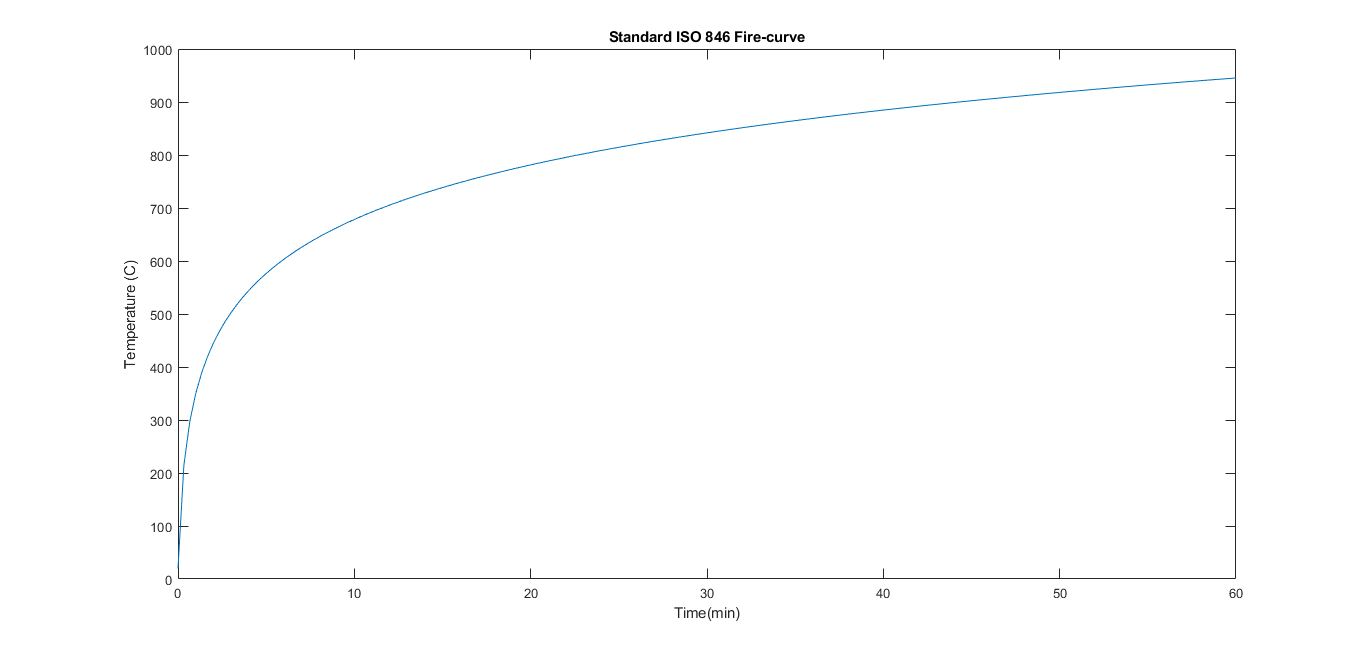
\includegraphics[width=\linewidth]{firecurve.png}
	\caption{Standard ISO fire curve TODO}
	\label{firecurve_fig}
	\end{figure}
	
	\subsection{Potential inaccuracies}
	As with most test everything is not always perfect. 
	In the data it was observed that two of the thermocouples broke during testing, this resulted in temperature with a magnitude of $10^{13}$. 
	That temperature is not possible as the highest ever recorded temperature reached was $4\text{x}10^{12}$ and that only occurred in a atomic explosion %(https://www.insidescience.org/news/hottest-temperature-universe-measured)% 
	This malfunction required that two of the depth measurements were no longer the average between nine samples but instead the average between eight.
	
	Another inaccuracy that could potentially influence the accuracy of the final result is the accuracy of the depth of the holes in which the thermocouples were placed. 
	As this was done by hand. %in the laboratory.
	
	There is also debate about the significance of the contribution of the timber burning to the temperature inside the furnace. 
	For the purposes of this project it will be assumed that the timber burning does not contribute to the temperature inside the furnace.
	
	The assumption that the panel is constantly at room temperature on the outside is also inaccurate as there is heat radiating from the panel that increases the temperature surrounding the panel.

\subsection{Results}



\begin{figure}[H]
	\label{measured_fig}
	\centering
	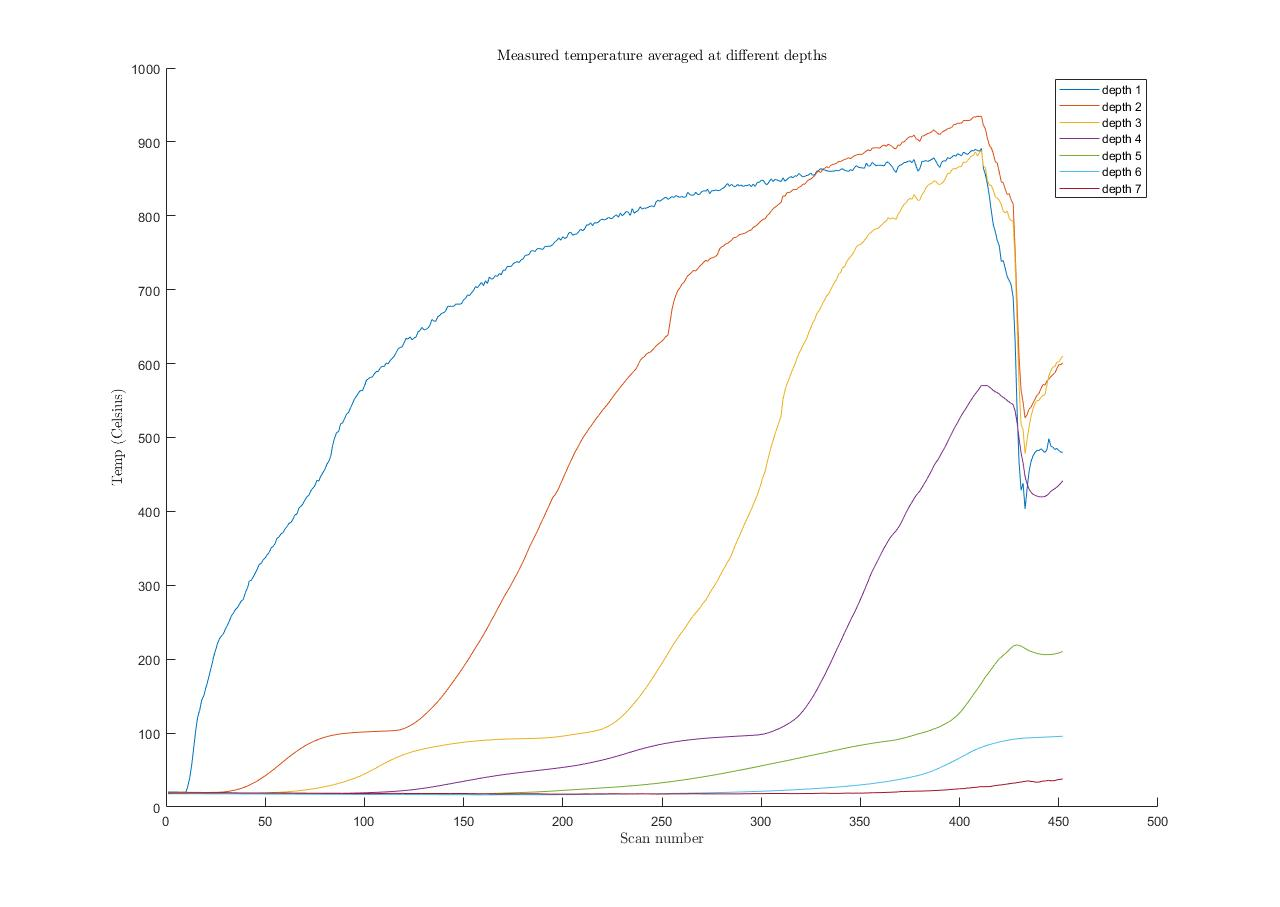
\includegraphics[width=5.5in,]{measured_data.jpg}
\end{figure}



\appendix%===========================================================

% \chapter{Concepts Generated}
\section{Concept I}
\section{Concept II}

%\include{App-B}
%\include{App-C}

\backmatter%=========================================================

\bibliography{USBibsample}

\end{document}
